\documentclass[12pt]{article}
 
\usepackage[margin=1in]{geometry}
\usepackage{amsmath,amsthm,amssymb}
\usepackage{mathtools}
\DeclarePairedDelimiter{\ceil}{\lceil}{\rceil}
%\usepackage{mathptmx}
\usepackage{accents}
\usepackage{comment}
\usepackage{graphicx}
\usepackage{IEEEtrantools}
 \usepackage{float}
 
\newcommand{\N}{\mathbb{N}}
\newcommand{\Z}{\mathbb{Z}}
\newcommand{\R}{\mathbb{R}}
\newcommand{\Q}{\mathbb{Q}}
\newcommand*\conj[1]{\bar{#1}}
\newcommand*\mean[1]{\bar{#1}}
\newcommand\widebar[1]{\mathop{\overline{#1}}}


\newcommand{\cc}{{\mathbb C}}
\newcommand{\rr}{{\mathbb R}}
\newcommand{\qq}{{\mathbb Q}}
\newcommand{\nn}{\mathbb N}
\newcommand{\zz}{\mathbb Z}
\newcommand{\aaa}{{\mathcal A}}
\newcommand{\bbb}{{\mathcal B}}
\newcommand{\rrr}{{\mathcal R}}
\newcommand{\fff}{{\mathcal F}}
\newcommand{\ppp}{{\mathcal P}}
\newcommand{\eps}{\varepsilon}
\newcommand{\vv}{{\mathbf v}}
\newcommand{\ww}{{\mathbf w}}
\newcommand{\xx}{{\mathbf x}}
\newcommand{\ds}{\displaystyle}
\newcommand{\Om}{\Omega}
\newcommand{\dd}{\mathop{}\,\mathrm{d}}
\newcommand{\ud}{\, \mathrm{d}}
\newcommand{\seq}[1]{\left\{#1\right\}_{n=1}^\infty}
\newcommand{\isp}[1]{\quad\text{#1}\quad}
\newcommand*\diff{\mathop{}\!\mathrm{d}}

\DeclareMathOperator{\imag}{Im}
\DeclareMathOperator{\re}{Re}
\DeclareMathOperator{\diam}{diam}
\DeclareMathOperator{\Tr}{Tr}
\DeclareMathOperator{\cis}{cis}

\def\upint{\mathchoice%
    {\mkern13mu\overline{\vphantom{\intop}\mkern7mu}\mkern-20mu}%
    {\mkern7mu\overline{\vphantom{\intop}\mkern7mu}\mkern-14mu}%
    {\mkern7mu\overline{\vphantom{\intop}\mkern7mu}\mkern-14mu}%
    {\mkern7mu\overline{\vphantom{\intop}\mkern7mu}\mkern-14mu}%
  \int}
\def\lowint{\mkern3mu\underline{\vphantom{\intop}\mkern7mu}\mkern-10mu\int}




\newenvironment{theorem}[2][Theorem]{\begin{trivlist}
\item[\hskip \labelsep {\bfseries #1}\hskip \labelsep {\bfseries #2.}]}{\end{trivlist}}
\newenvironment{lemma}[2][Lemma]{\begin{trivlist}
\item[\hskip \labelsep {\bfseries #1}\hskip \labelsep {\bfseries #2.}]}{\end{trivlist}}
\newenvironment{exercise}[2][Exercise]{\begin{trivlist}
\item[\hskip \labelsep {\bfseries #1}\hskip \labelsep {\bfseries #2.}]}{\end{trivlist}}
\newenvironment{problem}[2][Problem]{\begin{trivlist}
\item[\hskip \labelsep {\bfseries #1}\hskip \labelsep {\bfseries #2.}]}{\end{trivlist}}
\newenvironment{question}[2][Question]{\begin{trivlist}
\item[\hskip \labelsep {\bfseries #1}\hskip \labelsep {\bfseries #2.}]}{\end{trivlist}}
\newenvironment{corollary}[2][Corollary]{\begin{trivlist}
\item[\hskip \labelsep {\bfseries #1}\hskip \labelsep {\bfseries #2.}]}{\end{trivlist}}

\newenvironment{solution}{\begin{proof}[Solution]}{\end{proof}}
 
\begin{document}
 
% --------------------------------------------------------------
%                         Start here
% --------------------------------------------------------------
\title{Math 122B Homework 1}
\author{Ethan Martirosyan}
\date{\today}
\maketitle
\hbadness=99999
\hfuzz=50pt
\section*{Problem 1}
\subsection*{Part A}
First, we find that
\[
\frac{1}{z^4+z^2} = \frac{1}{z^2(z^2+1)} = \frac{1}{z^2(z+i)(z-i)}
\] We find that $z = 0$ is a pole of order $2$ and that $z = \pm i$ are simple poles. Let us compute the residue of $1/(z^4+z^2)$ at $0$. Notice that
\[
\frac{\diff }{\diff z} \bigg[ z^2 \cdot \frac{1}{z^4 + z^2}\bigg] = \frac{\diff }{\diff z} \bigg[ \frac{1}{z^2 + 1}\bigg] = -\frac{2z}{(1+z^2)^2}
\]
so that
\[
\text{Res}\bigg(\frac{1}{z^4+z^2}; 0\bigg) = \frac{1}{(2-1)!} \frac{\diff }{\diff z} \bigg[ z^2 \cdot \frac{1}{z^4 + z^2}\bigg]\bigg|_{z=0}  =  -\frac{2\cdot 0}{(1+0^2)^2} = 0
\] Next, we will compute the residue of $1/(z^4+z^2)$ at $i$. Note that
\[
\frac{1}{z^4 + z^2} = \frac{\frac{1}{z^2(z+i)}}{z-i}
\] Letting $A(z) = 1/(z^2(z+i))$ and $B(z) = z-i$, we find that
\[
\text{Res}\bigg(\frac{1}{z^4+z^2}; i\bigg) = \frac{A(i)}{B^\prime(i)} = \frac{1}{i^2(i+i)} = -\frac{1}{2i}
\] Finally, we will compute the residue of $1/(z^4+z^2)$ at $-i$. Note that
\[
\frac{1}{z^4 + z^2} = \frac{\frac{1}{z^2(z-i)}}{z+i}
\] Letting $A(z) = 1/(z^2(z-i))$ and $B(z) = z+i$, we find that
\[
\text{Res}\bigg(\frac{1}{z^4+z^2}; -i\bigg) = \frac{A(-i)}{B^\prime(-i)} = \frac{1}{(-i)^2(-i-i)} = \frac{1}{2i}
\]
\subsection*{Part B}
Notice that
\[
\cot z = \frac{\cos z}{\sin z}
\] Last quarter, we showed that $\cot z$ has a simple pole at every integral multiple of $\pi$. Letting $A(z) = \cos z$ and $B(z) = \sin z$, we find that
\[
\text{Res}\bigg(\cot z; n \pi\bigg) = \frac{A(n\pi)}{B^\prime(n\pi)} = \frac{\cos(n\pi)}{\cos(n\pi)} = 1
\]
\subsection*{Part C}
Notice that
\[
\csc z = \frac{1}{\sin z}
\] Last quarter, we showed that $\csc z$ has a simple pole at every integral multiple of $\pi$. Letting $A(z) = 1$ and $B(z) = \sin z$, we find that
\[
\text{Res}\bigg(\csc z; n\pi\bigg) = \frac{A(n\pi)}{B^\prime(n\pi)} = \frac{1}{\cos(n\pi)} = \frac{1}{(-1)^n} = (-1)^n
\]
\subsection*{Part D}
Notice that the function has a simple pole at $z = 1$. Letting $A(z) = \exp(1/z^2)$ and $B(z) = z - 1$, we have
\[
\text{Res}\bigg(\frac{\exp(1/z^2)}{z-1}; 1\bigg) = \frac{A(1)}{B^\prime(1)} = \exp(1) = e
\] Furthermore, this function has an essential singularity at $z = 0$. Notice that
\[
\frac{\exp(1/z^2)}{z-1} = \exp(1/z^2) \cdot -\frac{1}{1-z} = \bigg(1 + \frac{1}{z^2} + \frac{1}{2z^4} + \frac{1}{6z^6}+\cdots\bigg)(-1-z-z^2-z^3 - \cdots)  
\] Multiplying this out, we find that the coefficient $C_{-1}$ is
\[
-1 - \frac{1}{2} - \frac{1}{6} - \cdots = -e + 1
\] so that
\[
\text{Res}\bigg(\frac{\exp(1/z^2)}{z-1}; 0\bigg) = -e + 1
\]
\subsection*{Part E}
Notice that $z^2 + 3z + 2 = (z+1)(z+2)$ so that
\[
\frac{1}{z^2 + 3z + 2}
\] has simple poles at $-1$ and $-2$. We may write
\[
\frac{1}{z^2 + 3z + 2} = \frac{\frac{1}{z+1}}{z+2}
\] Letting $A(z) = 1/(z+1)$ and $B(z) = z+2$, we have
\[
\text{Res}\bigg(\frac{1}{z^2 + 3z + 2}; -2\bigg) = \frac{A(-2)}{B^\prime(-2)} = -1
\] We may also write
\[
\frac{1}{z^2 + 3z + 2} = \frac{\frac{1}{z+2}}{z+1}
\] Letting $A(z) = 1/(z+2)$ and $B(z) = z+1$, we have
\[
\text{Res}\bigg(\frac{1}{z^2 + 3z + 2}; -1\bigg) = \frac{A(-1)}{B^\prime(-1)} = 1
\]
\subsection*{Part F}
The function $\sin(1/z)$ has an essential singularity at $z = 0 $. Notice that
\[
\sin \frac{1}{z} = \frac{1}{z} - \frac{1}{3!}\frac{1}{z^3} + \cdots
\] so that
\[
\text{Res}\bigg(\sin \frac{1}{z}; 0\bigg) = 1
\]
\subsection*{Part G}
Notice that $ze^{3/z}$ has an essential singularity at $z = 0$. We have
\[
z e^{3/z} = z\bigg(1 + \frac{3}{z} + \frac{3^2}{2z^2} + \cdots\bigg) = z + 3 + \frac{9}{2z} + \cdots
\] so that
\[
\text{Res}\bigg(z e^{3/z} ; 0\bigg) = \frac{9}{2}
\]
\subsection*{Part H}
Notice that
\[
z = \frac{-b \pm \sqrt{b^2 - 4ac}}{2a}
\] If $b^2 - 4ac \neq 0$, then the function has simple poles at
\[
\frac{-b \pm \sqrt{b^2 - 4ac}}{2a}
\] 
Let 
\[
\alpha = \frac{-b + \sqrt{b^2 - 4ac}}{2a} 
\] and
\[
\beta = \frac{-b - \sqrt{b^2 - 4ac}}{2a}
\]
In particular, we may write
\[
\frac{1}{az^2 + bz + c} = \frac{1}{a} \cdot \frac{1}{z- \alpha} \cdot \frac{1}{z - \beta}
\] 
Letting
\[
A(z) = \frac{1}{a} \cdot \frac{1}{z - \alpha}
\] and
\[
B(z) = z - \beta
\] we may write
\[
\frac{1}{az^2 + bz + c} = \frac{A(z)}{B(z)}
\] Then, we have
\[
\text{Res}\bigg(\frac{1}{az^2 + bz + c}; \beta \bigg) = \frac{A(\beta)}{B^\prime(\beta)} = \frac{1}{a} \cdot \frac{1}{\beta - \alpha} = -\frac{1}{\sqrt{b^2 - 4ac}}
\] Next, letting
\[
A(z) = \frac{1}{a} \cdot \frac{1}{z - \beta}
\] and 
\[
B(z) =  \frac{1}{z - \alpha}
\] we may write
\[
\frac{1}{az^2 + bz + c} = \frac{A(z)}{B(z)}
\] Then, we have
\[
\text{Res}\bigg(\frac{1}{az^2 + bz + c}; \alpha \bigg) = \frac{A(\alpha)}{B^\prime(\alpha)} = \frac{1}{a} \cdot \frac{1}{\alpha - \beta} = \frac{1}{\sqrt{b^2 - 4ac}}
\] Next, we must consider the case in which $b^2 - 4ac  = 0$. Then, there is a double pole at $z = b/2a$ and
\[
\frac{1}{az^2 + bz + c} = \frac{1}{a(z-b/2a)^2}
\] The residue is 
\[
\frac{1}{(2-1)!} \frac{\diff}{\diff z} (z-b/2a)^2 \cdot \frac{1}{a(z-b/2a)^2}
\] evaluated at $z = b/2a$. However, we note that
\[
\frac{\diff}{\diff z} (z-b/2a)^2 \cdot \frac{1}{a(z-b/2a)^2} = \frac{\diff}{\diff z} \frac{1}{a} = 0
\] so that
\[
\text{Res}\bigg(\frac{1}{az^2 + bz + c}; \frac{b}{2a} \bigg) = 0
\]
\newpage
\section*{Problem 2}
\subsection*{Part A}
The singularities of $\cot z$ are at the integral multiples of $\pi$. The only singularity of $\cot z$ in the circle $\vert z \vert = 1$ is at $0$. The residue of $\cot z$ at $0$ is $1$. Appealing to the Residue Theorem, we find that
\[
\int_{\vert z \vert = 1} \cot z \diff z = 2\pi i 
\]
\subsection*{Part B} The only singularities of $1/(z-4)(z^3-1)$ in the circle $\vert z \vert = 2$ are $w_k := e^{2k\pi i  / 3}$, where $k = 0, 1, 2$. Notice that
\[
\frac{1}{(z-4)(z^3 - 1)} = \frac{1}{(z-4)(z-w_0)(z-w_1)(z-w_2)}
\] so that
\[
\text{Res}\bigg(\frac{1}{(z-4)(z^3 - 1)}; w_0\bigg) = \frac{1}{(w_0 - 4)(w_0 - w_1)(w_0 - w_2)}
\] and
\[
\text{Res}\bigg(\frac{1}{(z-4)(z^3 - 1)}; w_1\bigg) = \frac{1}{(w_1 - 4)(w_1 - w_0)(w_1 - w_2)}
\] and
\[
\text{Res}\bigg(\frac{1}{(z-4)(z^3 - 1)}; w_2\bigg) = \frac{1}{(w_2 - 4)(w_2 - w_0)(w_2 - w_1)}
\] Using the Residue Theorem, we find that
\[
\int_{\vert z \vert = 2} \frac{\diff z}{(z-4)(z^3 - 1)}
\] is equal to
\[
2\pi i\bigg(\frac{1}{(w_0 - 4)(w_0 - w_1)(w_0 - w_2)} + \frac{1}{(w_1 - 4)(w_1 - w_0)(w_1 - w_2)} + \frac{1}{(w_2 - 4)(w_2 - w_0)(w_2 - w_1)} \bigg)
\]
\subsection*{Part C}
Notice that the only singularity of $\sin \frac{1}{z}$ is at $0$; the residue there is $1$. Appealing to the Residue Theorem, we find that
\[
\int_{\vert z \vert = 1} \sin \frac{1}{z} \diff z = 2\pi i 
\]
\subsection*{Part D}
The only singularity of $ze^{3/z}$ is at $0$; the residue there is $9/2$. Appealing to the Residue Theorem, we find that
\[
\int_{\vert z \vert = 2} ze^{3/z} \diff z = \frac{9}{2} \cdot 2 \pi i = 9 \pi i
\]
\newpage
\section*{Problem 3}
Let $C$ be the unit circle. Notice that the only singularity of $1/(1-e^{-z})^n$ in $C$ is $0$ (the singularities of $1/(1-e^{-z})^n$ are at the integral multiples of $2\pi i$). By the Residue Theorem, we find that
\[
2\pi i \text{Res}\bigg(\frac{1}{(1-e^{-z})^n}; 0\bigg) = \int_C \frac{\diff z}{(1-e^{-z})^n}
\] Let $w =  1 - e^{-z}$. Then we have $\diff w  = e^{-z} \diff z$ so that
\[
\diff z = \frac{\diff w}{e^{-z}} = \frac{\diff w}{1-w}
\] Let $L$ denote the image of $C$ under $w(z) = 1-e^{-z}$.  Then, we have
\[
\int_C \frac{\diff z}{(1-e^{-z})^n} = \int_L \frac{\diff w}{w^n(1-w)}
\] The only singularities of $1/(w^n(1-w))$ are $0$ and $1$. In the below image, we can see that $L$ encloses $0$ but not $1$:
 \begin{figure}[H]
\centering
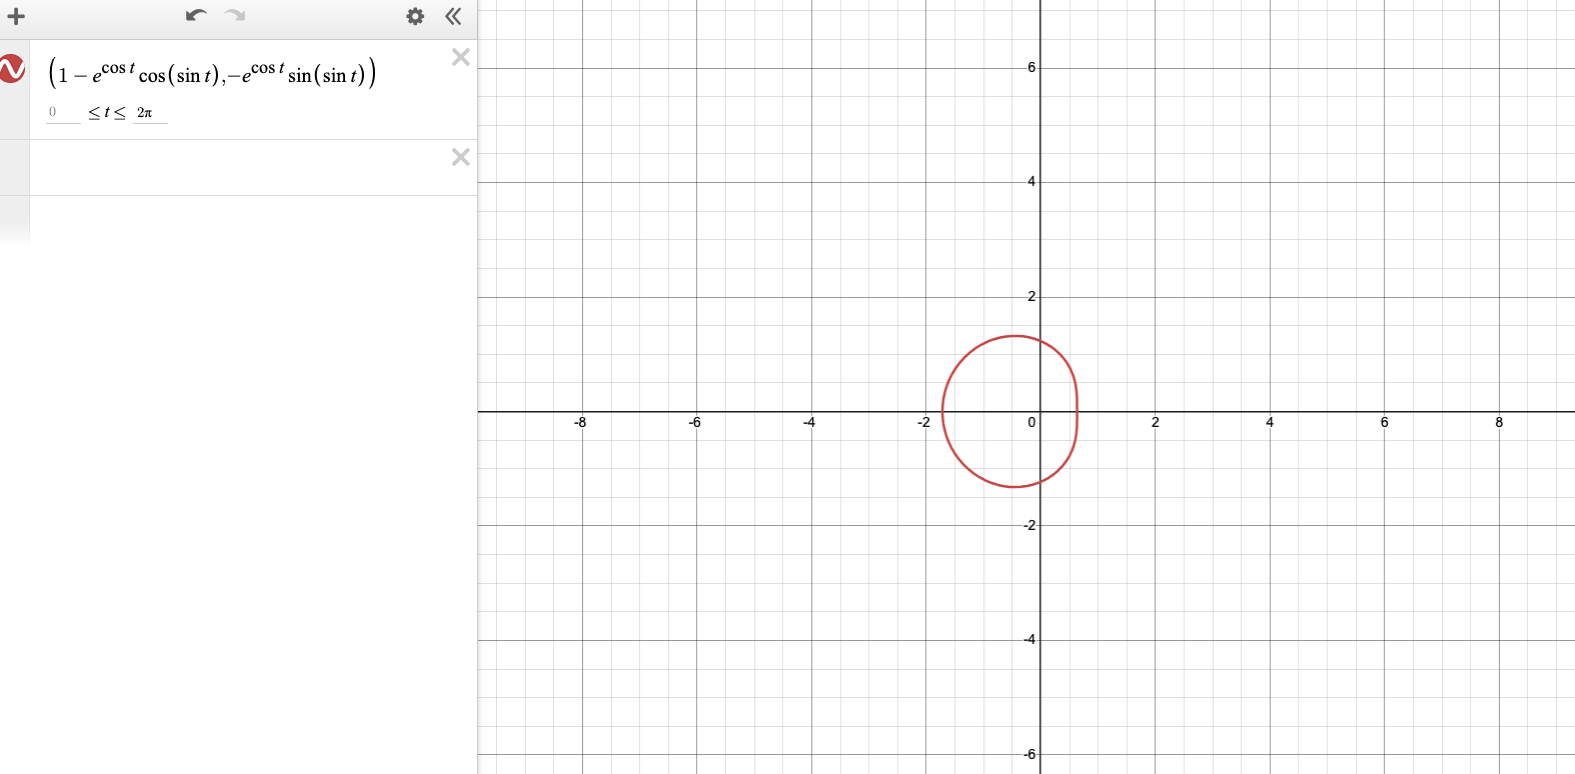
\includegraphics[width=\textwidth]{Image1}
\end{figure}
\noindent Thus, appealing to the Residue Theorem again, we have
\[
\int_L \frac{\diff w}{w^n(1-w)} = 2\pi  i \text{Res}\bigg( \frac{1}{w^n(1-w)}; 0 \bigg)
\] Notice that
\[
\frac{1}{w^n(1-w)} = \frac{1}{w^n} \cdot \frac{1}{1-w}  = \frac{1}{w^n}(1+w+w^2 +\cdots )
\] so that 
\[
\text{Res}\bigg( \frac{1}{w^n(1-w)}; 0 \bigg) = 1
\] Thus, we deduce that
\[
2\pi i \text{Res}\bigg(\frac{1}{(1-e^{-z})^n}; 0\bigg) = 2\pi  i \text{Res}\bigg( \frac{1}{w^n(1-w)}; 0 \bigg) = 2\pi i 
\] so that
\[
\text{Res}\bigg(\frac{1}{(1-e^{-z})^n}; 0\bigg) = 1
\]

\newpage
\section*{Problem 4}
Notice that
\[
\bigg(z+\frac{1}{z}\bigg) = \frac{z^2+1}{z}
\] Then, we have
\[
\bigg(\frac{z^2+1}{z}\bigg)^{2m+1} = \frac{(z^2+1)^{2m+1}}{z^{2m+1}}
\] By the Binomial Theorem, we have
\[
(z^2+1)^{2m+1} = \sum_{j=0}^{2m+1} \binom{2m+1}{j} z^{2j}
\] Then, we have
\[
\frac{(z^2+1)^{2m+1}}{z^{2m+1}} = \sum_{j=0}^{2m+1} \binom{2m+1}{j} z^{2j-2m-1}
\] Thus, we have
\[
\int_{\vert z \vert = 1} (z+1/z)^{2m+1} \diff z = \sum_{j=0}^{2m+1}  \binom{2m+1}{j} \int_{\vert z \vert = 1} z^{2j-2m-1} \diff z
\] We know that
\[
\int_{\vert z \vert = 1} z^n \diff z 
\] is $2\pi i$ if $n = -1$ and $0$ otherwise. Thus, we find that
\[
\int_{\vert z \vert = 1} z^{2j-2m-1} \diff z
\] is $0$ if $j \neq m$ and $2\pi i$ if $j = m$ so that
\[
\int_{\vert z \vert = 1} (z+1/z)^{2m+1} \diff z = \sum_{j=0}^{2m+1}  \binom{2m+1}{j} \int_{\vert z \vert = 1} z^{2j-2m-1} \diff z = 2\pi i \binom{2m+1}{m}
\]
\end{document} 